\chapter{Testing functional and nonfunctional requirements in User Requirements Notation}
%--------------------------------------------------------------------------------%
%--------------------------------------------------------------------------------%
\section{Introduction}

Software testing is a key-activity for software quality management to ensure that the developed software behaves as expected. The anticipated behavior and requirements can be defined in the User Requirements Notation. 

The User Requirements Notation is a notation for modeling, analyzing, and controlling the correctness and completeness of functional and non-functional requirements. It is divided into two notations: the Use Case Map for the functional and the Goal-oriented Requirements Language for the non-functional requirements. User Requirements Notation is a good starting point for several reasons: it is scenario-based, requirements oriented, independent of the implementation, models functional and non-functional requirements, and is easy to add in the development process. Independence from the implementation is essential; even though code-based testing is an excellent test method, the stakeholder's requirements will not be tested.

A serious risk of manual test generation is a high probability for false test cases. This is due to the test cases' repetition, whereas only the input and output data change. Therefore, the test logic is the same, and the developer tends to copy and paste the test cases, which can lead to copying the code and the test logic mistakes. In this case, writing manual tests is time-wasting for the developer.  To avoid these risks and use the developer's time wisely, it is essential to automate the test case generation process.

This chapter focuses on the article \textit{"Scenario-Based Validation Beyond the User Requirements Notation" by Arnold et al.}\cite{ArnoldCorriveauShi2010} and the article \textit{"Transforming Workflow Models into Automated End-to-End Acceptance Test Cases" by Boucher and Mussbacher}\cite{BoucherMussbacher2017}. The primary was provided by the supervisors, whereas the second was selected after the literature research. Further information about the literature research is presented in \autoref{topic08:sectionLiteratur}. In \autoref{topic08:sectionApproach1}, the first paper's approach is described and applied, which will also be the case in the \autoref{topic08:sectionApproach2} regarding the second paper. In the penultimate \autoref{topic08:sectionComparison}, the two approaches will be compared based on a synthesis matrix, and the chapter will be completed with a conclusion.

Please visit the glossary to get familiar with: functional requirements (FR), non-functional requirements (NFR), User Requirements Notation (URN), Use Case Map (UCM), Goal-oriented Requirements Language (GRL), acceptance test, test cases, stakeholders, scenario, implementation under test (IUT), JUnit testing Framework.
%--------------------------------------------------------------------------------%
%--------------------------------------------------------------------------------%
\section{Literature Search}
\label{topic08:sectionLiteratur}

\subsubsection{Research planning} 

\textbf{Research question:} The research question is "Which approaches for the systematic generation of tests for functional and non-functional requirements from the User Requirements Notation exist?"

\textbf{Snowballing:} For the snowballing research, the given paper \textit{"Scenario-Based Validation Beyond the User Requirements Notation" by Arnold et. al} will be used. The paper is found on IEEE Xplore.\footnote{https://ieeexplore.ieee.org/document/5475050} On IEEE Xplore, one can see that the article referenced 29 articles and has been referenced by four. 

\textbf{Search term based search:} The search was done for the terms "User Requirements Notation" and "test" in order to answer the research question. If the papers do not include in \textit{"All Metadata"} those two terms, they are not useful to answer the research question.

\textbf{Research Sources:} IEEE Xplore\footnote{https://ieeexplore.ieee.org/Xplore/home.jsp}, ACM\footnote{https://dl.acm.org/}. These two are the primary scientific associations for computer science and include almost all essential and verified scientific papers.

\textbf{Relevance criteria:} The paper should deal with an approach for the systematic generation of tests for functional and non-functional requirements from the User Requirements Notation. In detail:
\begin{itemize}
	\itemsep-1em
	\item User Requirements Notation: for our research question, the requirements must be written down in the User Requirements Notation
	\item functional and non-functional requirements: both the functional and non-functional requirements should be tested 
	\item systematic generation of test: the goal is that the tests are systematically generated
	\item extra: the article should not be by the same authors
\end{itemize}

\subsubsection{Research results (\autoref{tab:08_research})}

\textbf{Backward snowballing:} \textit{Arnold et al.} have 29 references. 13 of the 29 references can be ignored because they are only references for definitions and links to websites for more information. Thus, 16 articles are helpful to address the research question, which is why all 16 papers are analyzed and checked if the relevance criteria are met. Unfortunately, none of them meets all criteria; either the articles deal with User Requirements Notation and functional and non-functional requirements or the systematic generation of tests. 

\textbf{Forward snowballing:} The article from \textit{Arnold et al.} was published in the year 2010, according to IEEE Xplore. Since then, only four articles referenced \textit{"Scenario-Based Validation Beyond the User Requirements Notation"}. One of the four is a summary of 35 articles - another is written by one of the authors of the given paper, and the third does not meet any criteria. One article left \textit{"Transforming Workflow Models into Automated End-to-End Acceptance Test Cases" from Boucher and Mussbacher}. The last article deals with the systematic generation of tests for functional requirements from the User Requirements Notation. However, the generation of tests for non-functional requirements is not addressed by \textit{Boucher and Mussbacher}, an article that meets all the decision criteria was not found, which is why the last paper was chosen for future evaluation.

\textbf{Search term based search:} On IEEE Xplore, one searches with \textit{"(("All Metadata":"user requirements notation") AND "All Metadata":test)"} and gets five results. One result is the given article \textit{"Scenario-Based Validation Beyond the User Requirements Notation"} and another the article \textit{"Transforming Workflow Models into Automated End-to-End Acceptance Test Cases"} from the forward snowballing, so we get three new papers. Unfortunately, none of the three papers meets all criteria. On ACM, one searches with \textit{"[Abstract: "user requirements notation"] AND [All: test]"} and gets seven results. One of them was \textit{"Transforming Workflow Models into Automated End-to-End Acceptance Test Cases"}, and of the remaining six papers, none meets all criteria.

\begin{table}[h]
	\caption{Literature Research Documentation.}
	\begin{longtable}{|p{1cm}|p{1.5cm}|>{\raggedright}p{2cm}|>{\raggedright}p{3.7cm}|p{1.3cm}|p{1.4cm}|p{0.7cm}|}
		\hline
		\textbf{Source} & \textbf{Date} & \textbf{Restrictions} & \textbf{Term} & \textbf{Results} & \textbf{Relevant} & \textbf{Used}\\
		\hline
		IEEE$^*$ & 22.11.2020 & none & backward snowballing & 16(29) & 0 & none \\
		\hline
		IEEE$^*$ & 22.11.2020 & none & forward snowballing & 4 & 1 & $\nabla$ \\
		\hline
		IEEE$^*$ & 22.11.2020 & none & (("All Metadata":"user requirements notation") AND "All Metadata":test) & 3(5) & 1 & none\\
		\hline
		ACM$^\dagger$ & 22.11.2020 & urn: abstract & [Abstract: "user requirements notation"] AND [All: test] & 6(7) & 1 & none \\
		\hline
	\end{longtable}
	\textit{*: https://ieeexplore.ieee.org/Xplore/home.jsp \quad $\dagger$: https://dl.acm.org/ \quad $\nabla$: \cite{BoucherMussbacher2017}}
	\label{tab:08_research}
\end{table}
%--------------------------------------------------------------------------------%
%--------------------------------------------------------------------------------%
\newpage
\section{Scenario-Based Validation Beyond the User Requirements Notation\cite{ArnoldCorriveauShi2010}}
\label{topic08:sectionApproach1}

\subsection{Description}

\textit{Dave Arnold} and \textit{Jean Pierre Corriveau} of Carleton University and \textit{Wei Shi} of University of Ontario Institute of Technology wrote the paper \textit{Scenario-Based Validation Beyond the User Requirements Notation}, which was published in 2010 by IEEE in the 21st Australian Software Engineering Conference.

The authors want to automate the generation, the execution, and the evaluation of test cases for functional and non-functional requirements from the User Requirements Notation (see \autoref{fig:08_flowOf1}). The automatic test generation should be independent of the implementation under test (IUT), but the test case executability on the IUT must be secured. Additionally, \textit{Arnold et al.} require traceability between the test cases and the IUT in order to find out where the error occurs. To achieve these goals, they define the "testable requirements model" (TRM), which supports traceability by connecting its elements with the IUT elements and also connects the stakeholders with the developers. Moreover, the TRM can handle functional and non-functional requirements, support metric evaluators to evaluate the non-functional requirements, and statistic checks for the statistical analysis. TRM is textual and must be written in its requirements specification language with the name "Another Contract Language". The transformation from the User Requirements Notation, in detail the Use Case Map and Goal-oriented requirements Notation, to the TRM is not automated. This process requires a person who is familiar with the Another Contract Language's semantic, the test case generation process, and the binding process between the TRM and the IUT. The authors note that this process is straightforward because of the semantic similarity between the URN and the TRM. After the TRM has been created, the developer can start the "Validation Framework" (VF), which needs the TRM and the IUT as input. The VF's first step is to call the "automated binding engine", which automates the binding process between the TRM and the IUT by linking corresponding elements and methods. This process must be done to enable the test cases' executability on the IUT and traceability between the test cases and the IUT. The VF's next step is to start the IUT and run the statistic checks and the metric evaluator. After that, the VF can test the IUT with the already created test cases and check if it behaves as expected. The VF stores information about the input of the test case, the behavior of the IUT, the difference to the expected behavior, if necessary, and the points where the IUT begins to behave unexpectedly as well as the results. All of this information will be written in the "contract evaluation report".

\begin{figure}
	\centering
	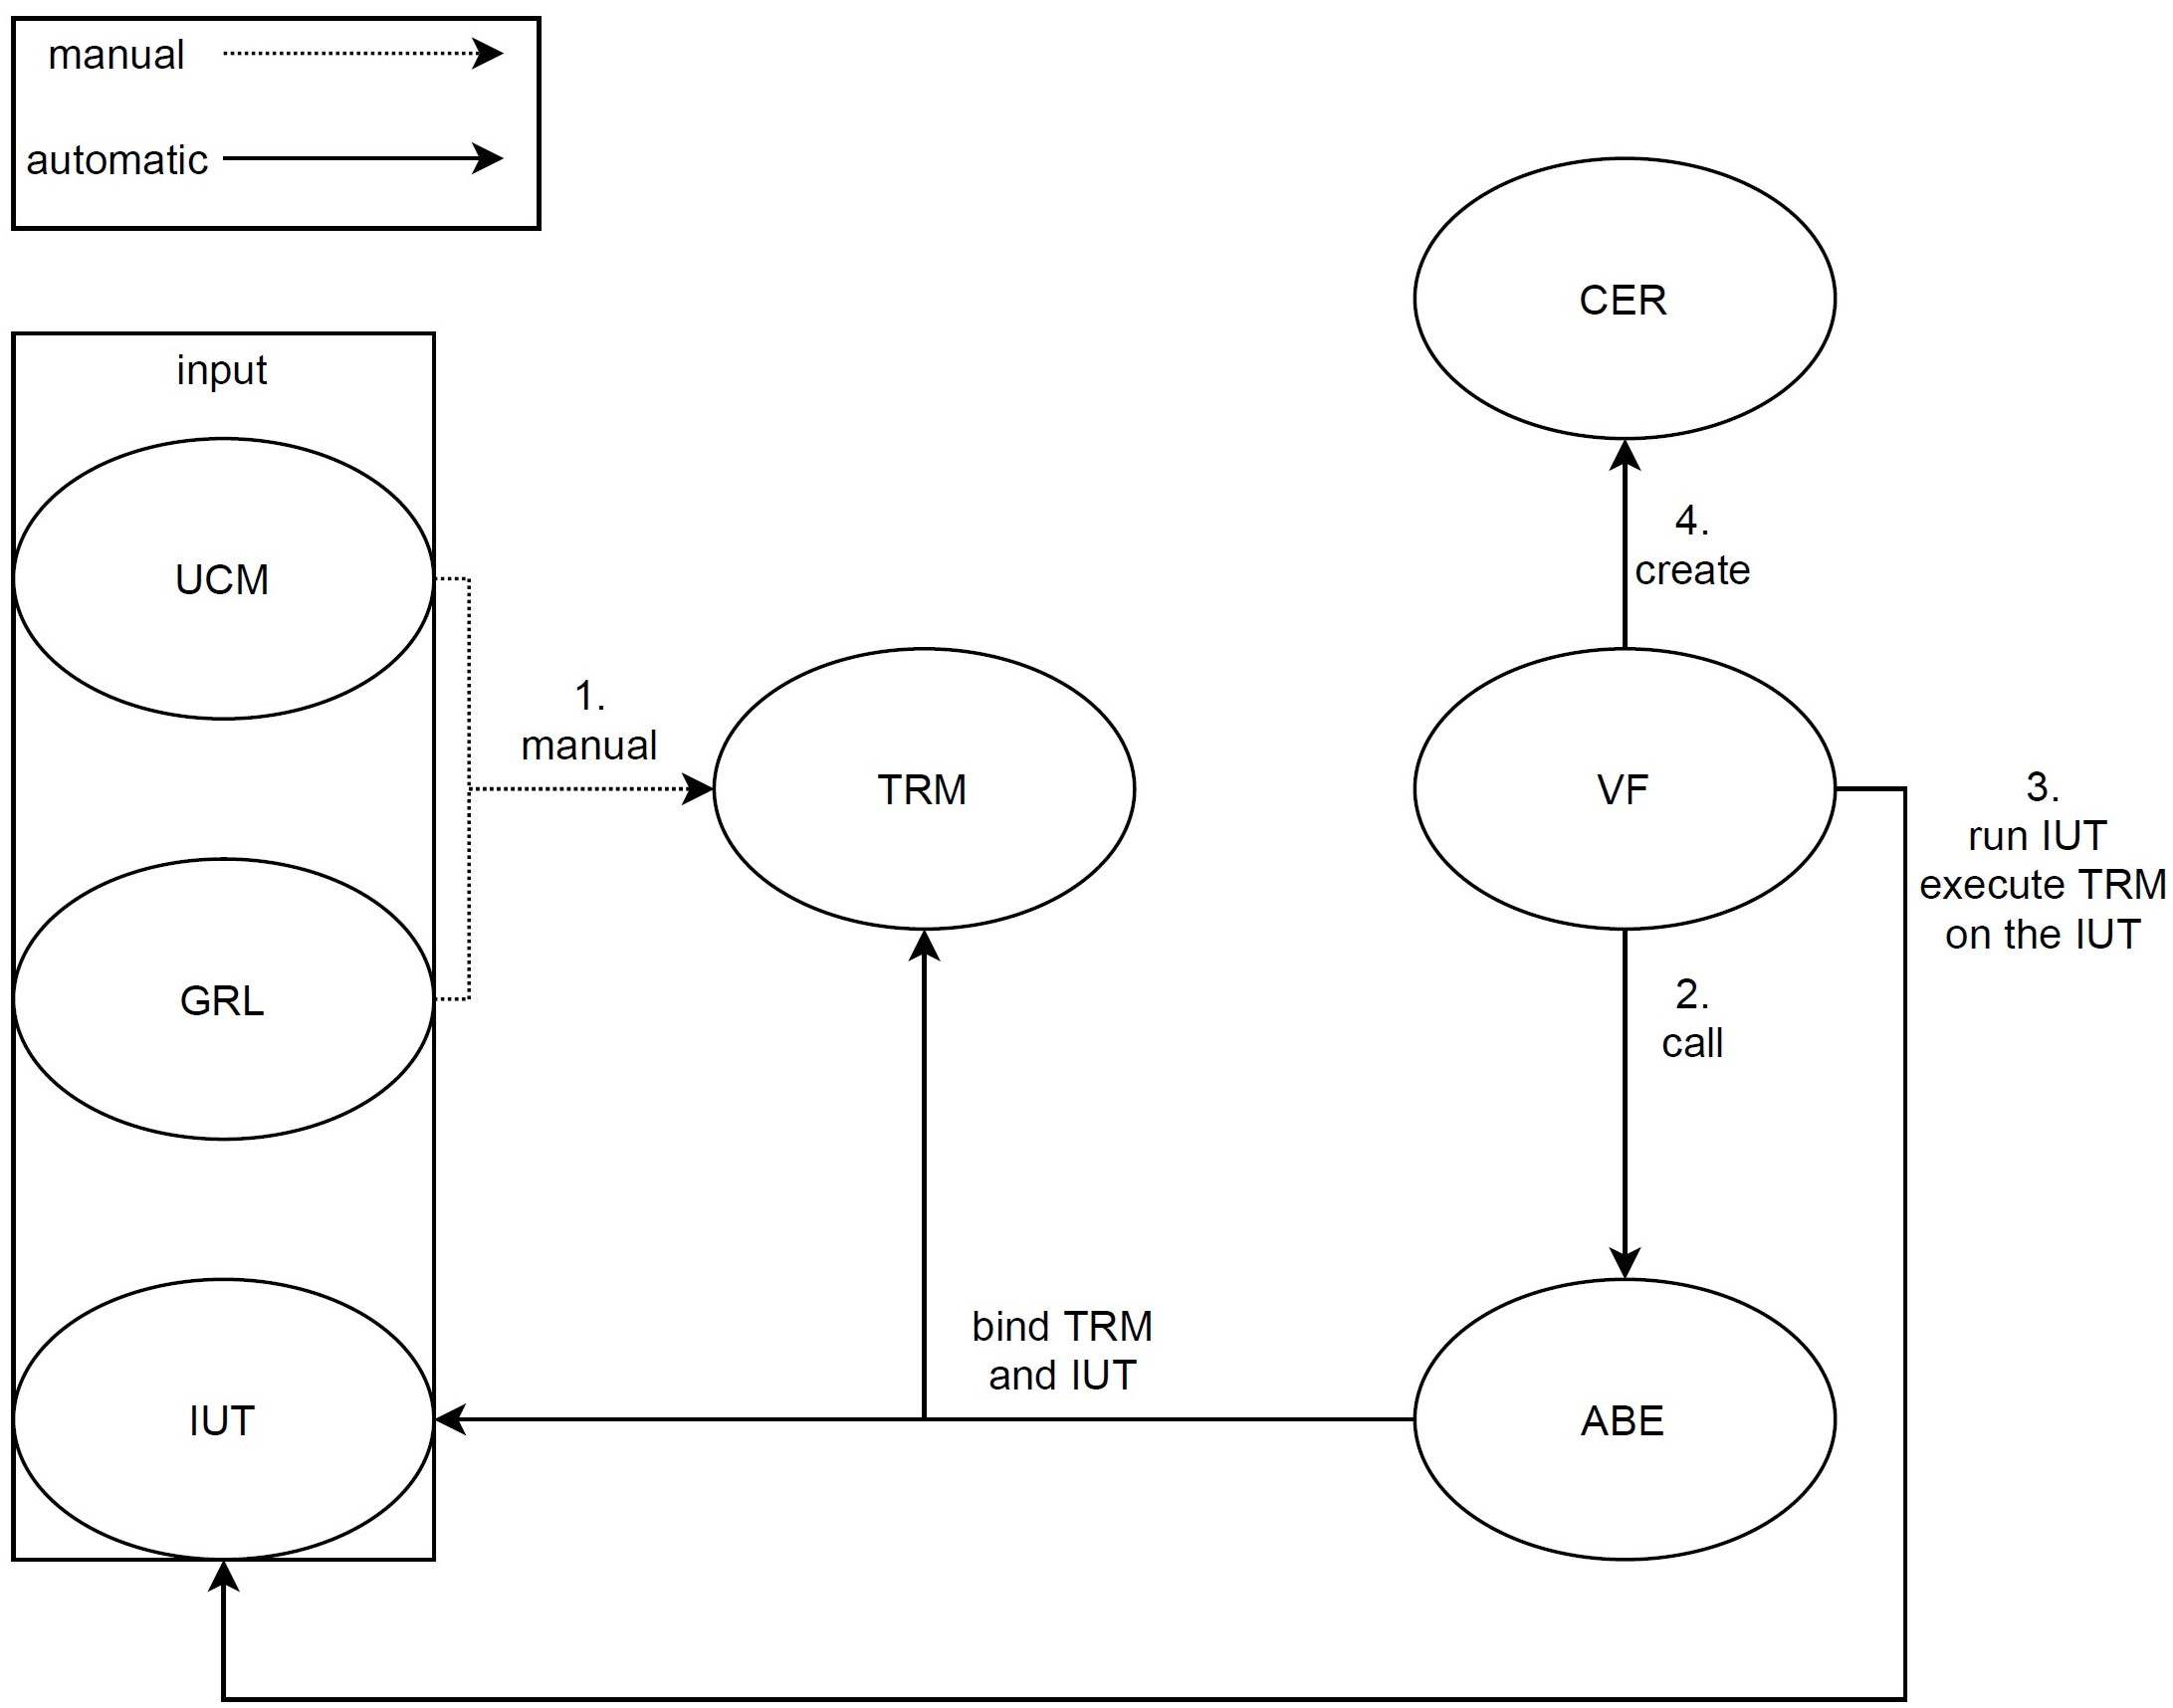
\includegraphics[scale=0.4]{../images/08/08_controllFlow1.jpg} 
	\caption{Flow of approach 1}
	\label{fig:08_flowOf1}
\end{figure}

%--------------------------------------------------------------------------------%
\newpage
\subsection{Application}
In this section, the approach by \textit{Arnold et al.} applies to the Software \textit{Movie Manager}.
\subsubsection{Input: User Requirements Notation.}
The functional requirements in the Use Case Maps Notation and non-functional requirements in the Goal-oriented Requirements Language are in view in \autoref{fig:08_UCMMovieManagement} and \autoref{fig:08_GRLMovieManagement}. \autoref{fig:08_UCMMovieManagement} describes which functions can execute in the IUT. \autoref{fig:08_GRLMovieManagement} describes which goals the functions achieve and on which soft goal it has an influence. 
\begin{figure}[h]
	\centering
	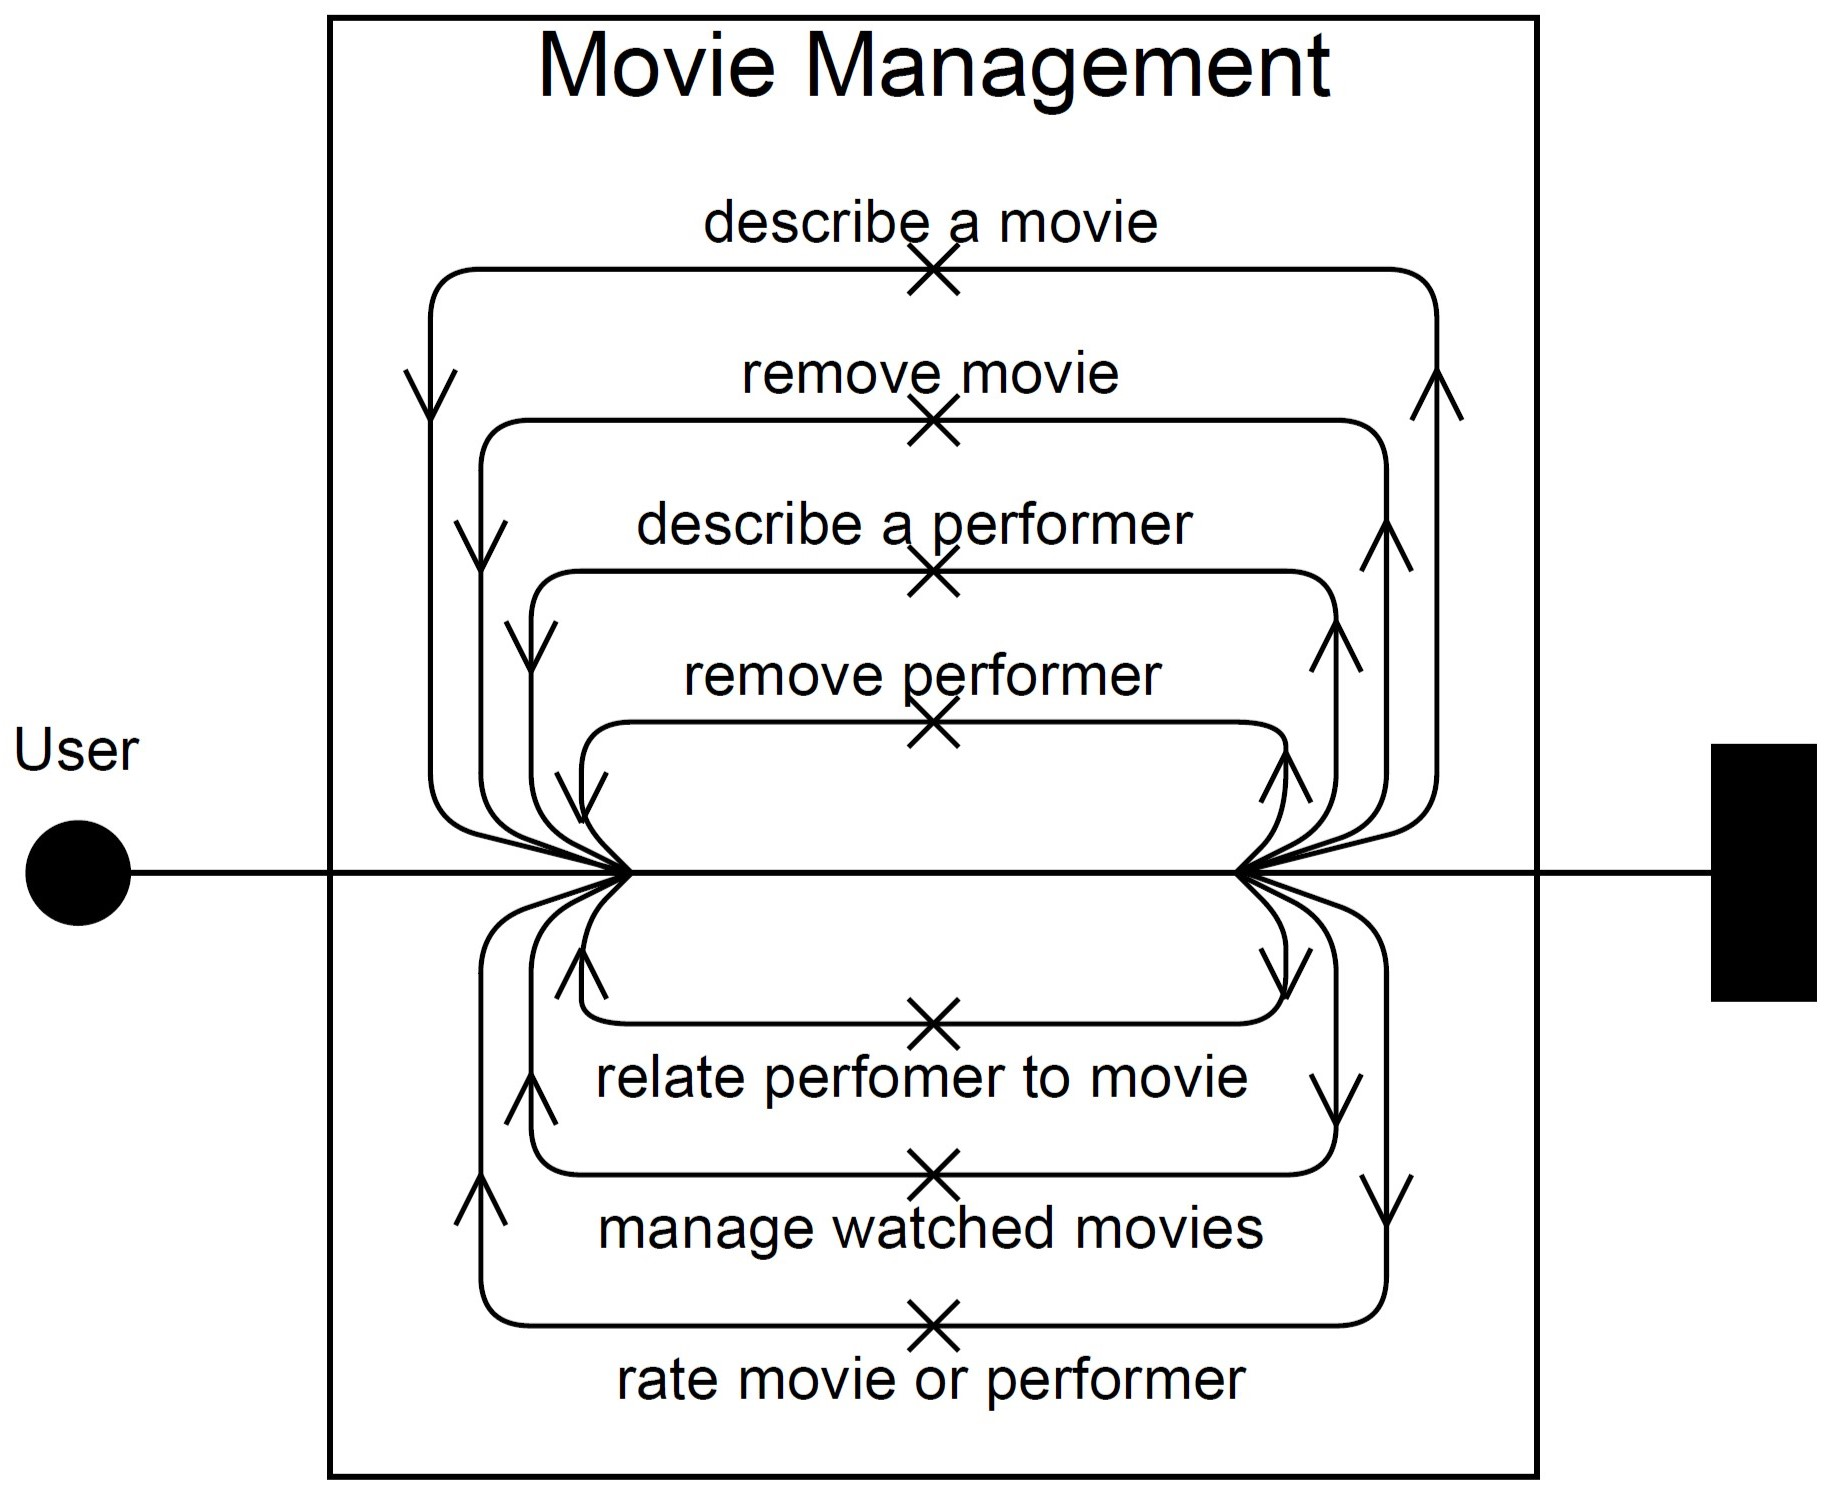
\includegraphics[scale=0.29]{../images/08/08_UCMMovieManagement.jpg} 
	\caption{Functional Requirements in Use Case Maps Notation}
	\label{fig:08_UCMMovieManagement}
\end{figure}
\begin{figure}[h]
	\centering
	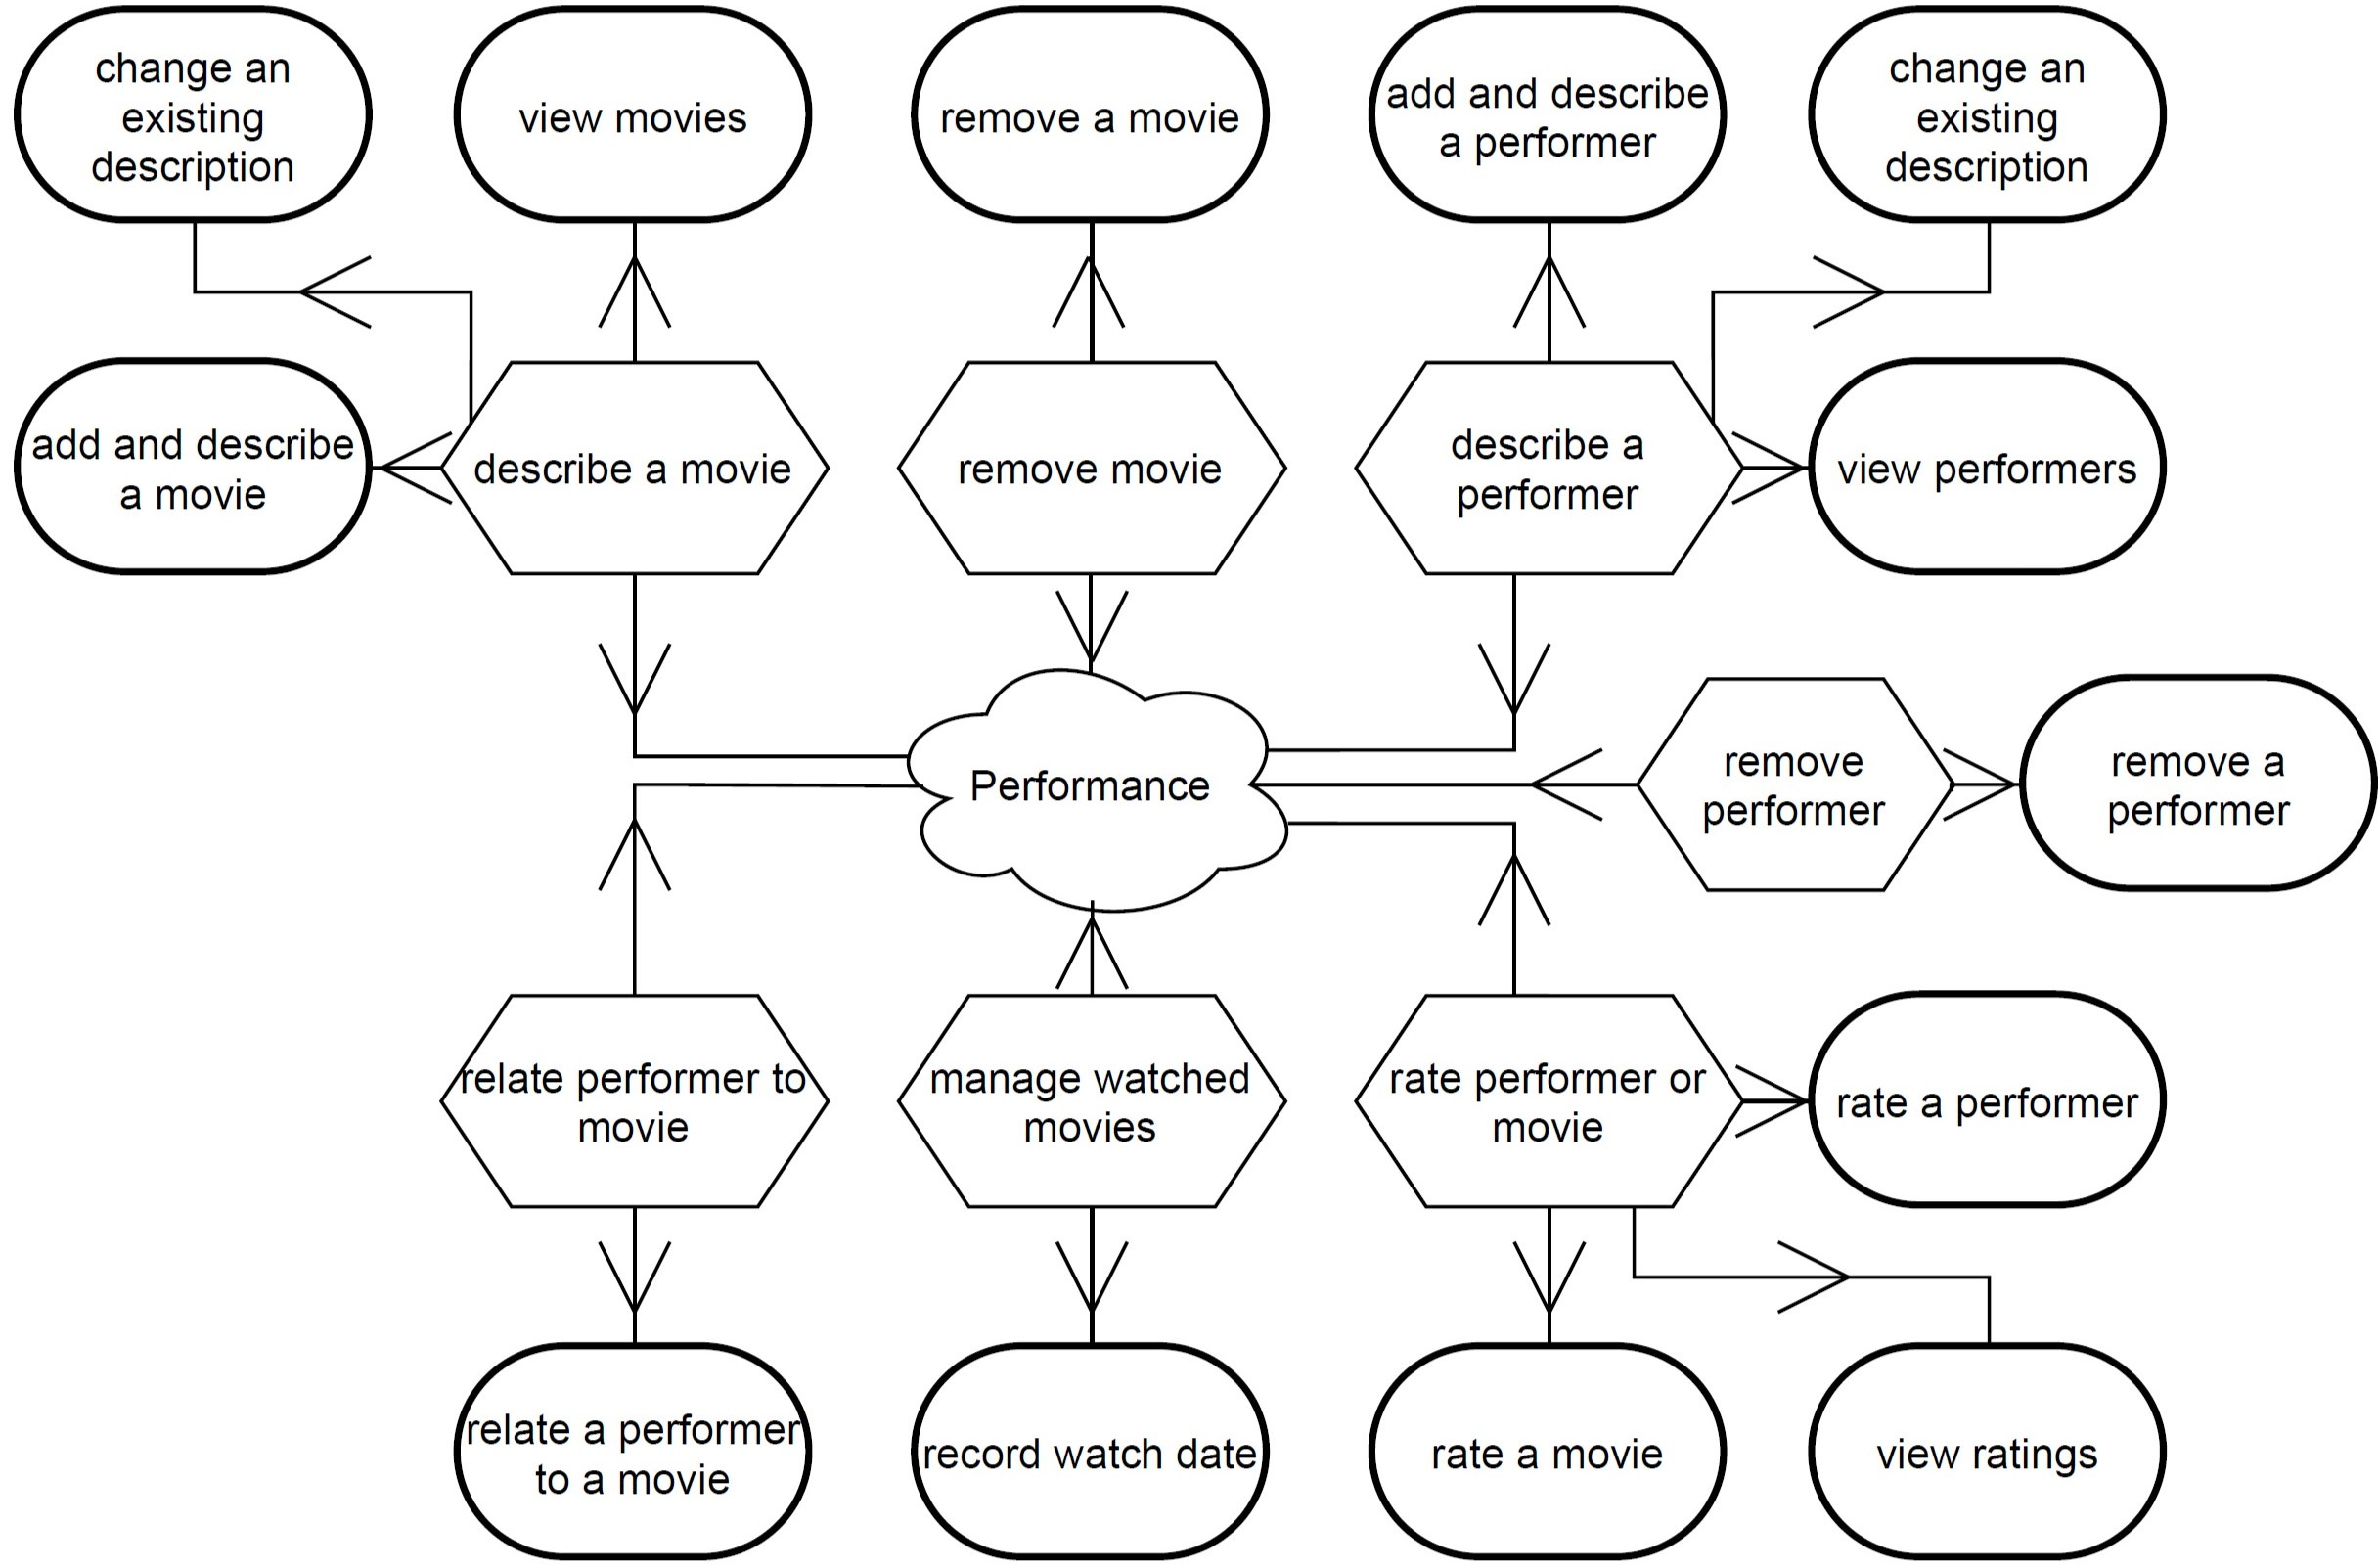
\includegraphics[scale=0.4]{../images/08/08_GRLMovieManagement.jpg} 
	\caption{Non-functional Requirements in Goal-oriented Requirements Language}
	\label{fig:08_GRLMovieManagement}
\end{figure}

\subsubsection{First Step: Conversion URN to TRM}
For simplicity, the example will be limited to the system functions "Add Movie" and "Remove Movie". The non-functional requirement is "performance", and the question is how fast movies can be added and removed.

For clarity, this step is split up into two. First, the functional requirements convert to the TRM. The result is in \autoref{lst:08_TRM1}. In the TRM is for each function that should be tested one responsibility. The responsibility checks the preconditions, executes the IUT's method, updates global variables if necessary, and checks the postconditions. Help functions and help variables for the responsibilities are defined as observability and scalar. 

\lstinputlisting[caption={TRM}, label={lst:08_TRM1}]{../images/08/08_ContractMovieManagment_UCM.java}

Second, the non-functional requirements must be added to \autoref{lst:08_TRM1}. The result is in \autoref{lst:08_TRM2}. Two new scalars, \textit{add\_timer} and \textit{remove\_timer}, are needed to evaluate the performance. This timer must start before and stop after the execution in the responsibility. Also, two scenarios are needed. \textit{AddRemoveMovie} define the behavior of an element in the \textit{Contract} and the \textit{Lifetime} define the lifetime of the \textit{Contract}. \textit{Reports} write the information in the CER and need the two \textit{Metric's} \textit{TimesToAddMovie} and \textit{TimesToRemoveMovie}.

\lstinputlisting[caption={TRM}, label={lst:08_TRM2}]{../images/08/08_ContractMovieManagment.java}

\subsubsection{Second Step: Run VF}

The VF first calls the ABE for the binding process between corresponding elements of the TRM and the IUT. Result in \autoref{tab:bindingTable}. The contract, all export types, all responsibilities, and all observabilities from the TRM need to link to the corresponding elements from the IUT. In the first column are the TRM elements, and in the third column the IUT elements.

\begin{table}[h] 
	\centering
	\begin{small}
		\caption{Binding table between TRM and IUT}
		\label{tab:bindingTable}
		\setlength{\tabcolsep}{1em}
		\begin{tabular}{>{\raggedright}p{3.5cm}| p{1.75cm}|>{\raggedright}p{5.8cm} |p{0.75cm} }
			\hline
			TRM element name & TRM type & IUT bindpoint & IUT type \\
			\hline
			\hline	
			MovieManagement & Contract & MovieManager & class\\
			\hline
			Movie & Exported Type & Movie MovieManger::Movie & class \\
			\hline
			Boolean HasMovie(Movie item) & Observability & bool MovieManager::Movie.HasItem (MovieManager::Movie) & Method \\
			\hline
			Void AddMovie(Movie item) & Responsibility & void  MovieManager::Movie.createMovie (MovieManager::Movie) & Method \\
			\hline
			Boolean RemoveMovie(Movie item) & Responsibility & void MovieManager::Movie.removeMovie (MovieManager::Movie) & Method \\
			\hline
		\end{tabular}
	\end{small}
\end{table}

After that, the VF starts the IUT, runs the TRM on the IUT, saves all information, and creates the CER.
%--------------------------------------------------------------------------------%
%--------------------------------------------------------------------------------%
\newpage
\section{Transforming Workflow Models into Automated End-to-End Acceptance Test Cases\cite{BoucherMussbacher2017}}
\label{topic08:sectionApproach2}

\subsection{Description}
\label{topic08:sectionApproach2Description}

\textit{Mathieu Boucher} and \textit{Gunter Mussbacher} of McGill University wrote the paper \textit{Transforming Workflow Models into Automated End-to-End Acceptance Test Cases}, which was published in 2017 by IEEE/ACM in the 9th International Workshop on Modelling in Software Engineering (MiSE).

The authors in this paper want to generate acceptance tests from the User Requirements Notation. Since \textit{Boucher} and \textit{Mussbacher} focus on the functional requirements, they only need the Use Case Maps (see \autoref{fig:08_flowOf2}). These test cases will be executed with the "JUnit Testing Framework", which will be discussed later. In order to enable this, the Use Case Maps must be extended. The input data, the expected output, a description of the behavior, and the test logic with postconditions are needed. In greater detail, the scenario groups, scenario definition, start- and endpoints, and responsibilities have to be included. Scenario groups contain the name of the data/class, global settings and information for the starting and ending process, and global variables for the tests. A scenario group includes several scenario definitions, which correspond to a use case. The scenario definitions' inputs consist of the data type (e.g., boolean, integer, string, etc.) and the values. Start points define the system state before the scenario starts. Responsibilities describe an action in the scenario and are connected with the system code, whereas endpoints define the system state after the scenario ends. 

The test case's extent depends on the number of responsibilities that the traversal mechanism meets during the traversal. If the mechanisms only meet one responsibility, the test cases are like Unit Tests. If the mechanisms meet many responsibilities, the test cases are similar to acceptance test cases. After the Use Case Maps diagram is extended, the traversal mechanism can analyze the diagram, which means it is traveling through the Use Case Map, from the start point to an endpoint by visiting the responsibilities, which creates the test cases automatically. For each scenario definition, the mechanism will generate a test case skeleton, which is used with the input combinations to create specific acceptance test cases. Thus, one has one test case for each input combination. 

The input combinations are determined according to the paper with boundary value analysis and Myer's test selection heuristics. In further detail, for instance the input data is from type integer and has the interval [-10,20], which results in eight test cases, two invalid \{-11, 21\} and six valid \{-10,-9, 0, 5, 19, 20\}. In \textit{"TABLE I. SUPPORTED TYPES FOR INPUT VARIABLES"} on page four of the paper \cite{BoucherMussbacher2017}, one can find information about creating the test cases from the input values for all supported data types. If there is more than one input data for a scenario definition, the values' selection is based on Myer's test selection heuristics. They create one test case for each invalid value, and the other input values must be valid. Therefore, one can focus on each invalid value. Each input's valid values are combined for the rest, so all the valid values are tested at least once. The test cases end with comparing the output and the system's behavior with the expected output and behavior. If all test cases are created, the "JUnit Testing Framework" can execute the test cases on the software and show which are successful and which not.

\begin{figure}[h]
	\centering
	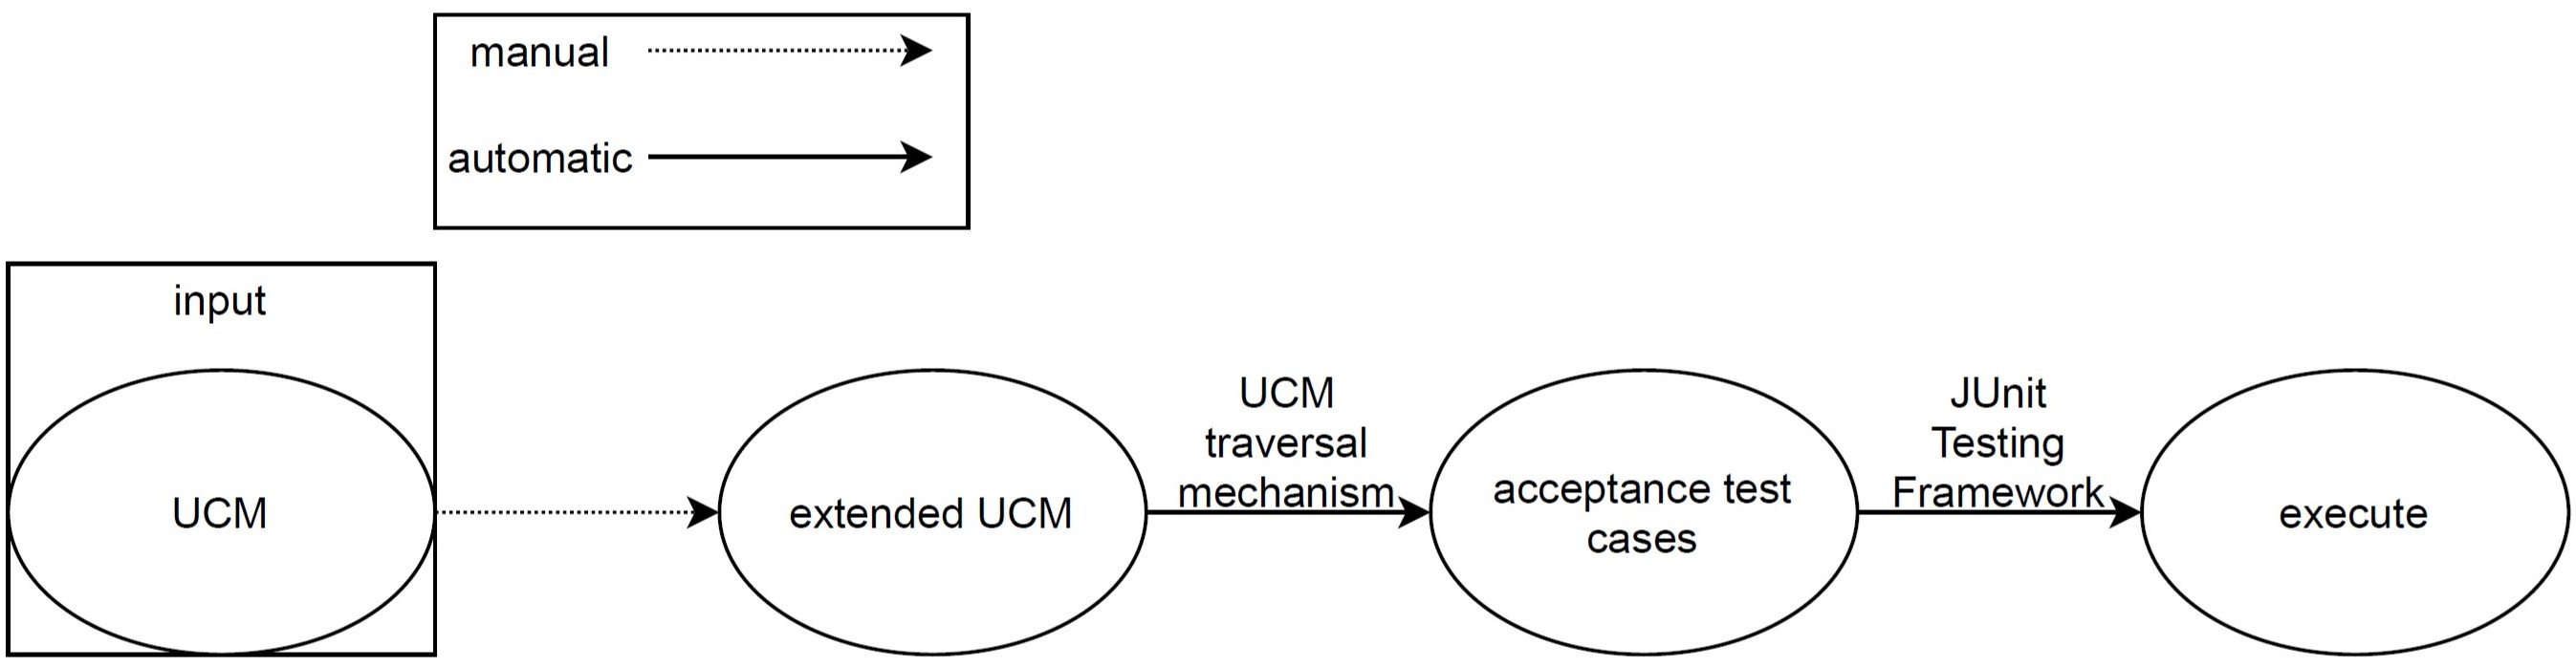
\includegraphics[scale=0.4]{../images/08/08_controllFlow2.jpg} 
	\caption{Flow of approach 2}
	\label{fig:08_flowOf2}
\end{figure}
%--------------------------------------------------------------------------------%
\subsection{Application}

In this section, the approach by \textit{Boucher and Mussbacher} applies to the Software \textit{Movie Manager}.

\subsubsection{Input: Use Case Map}

For simplicity, the example will be limited to the system function "add and describe a movie". The Functional Requirements in the Use Case Maps Notation is in view in figure \ref{fig:08_UCMAddAndDescribeMovie}. \autoref{fig:08_UCMAddAndDescribeMovie} describes which functions can execute in the IUT.

\begin{figure}[h]
	\centering
	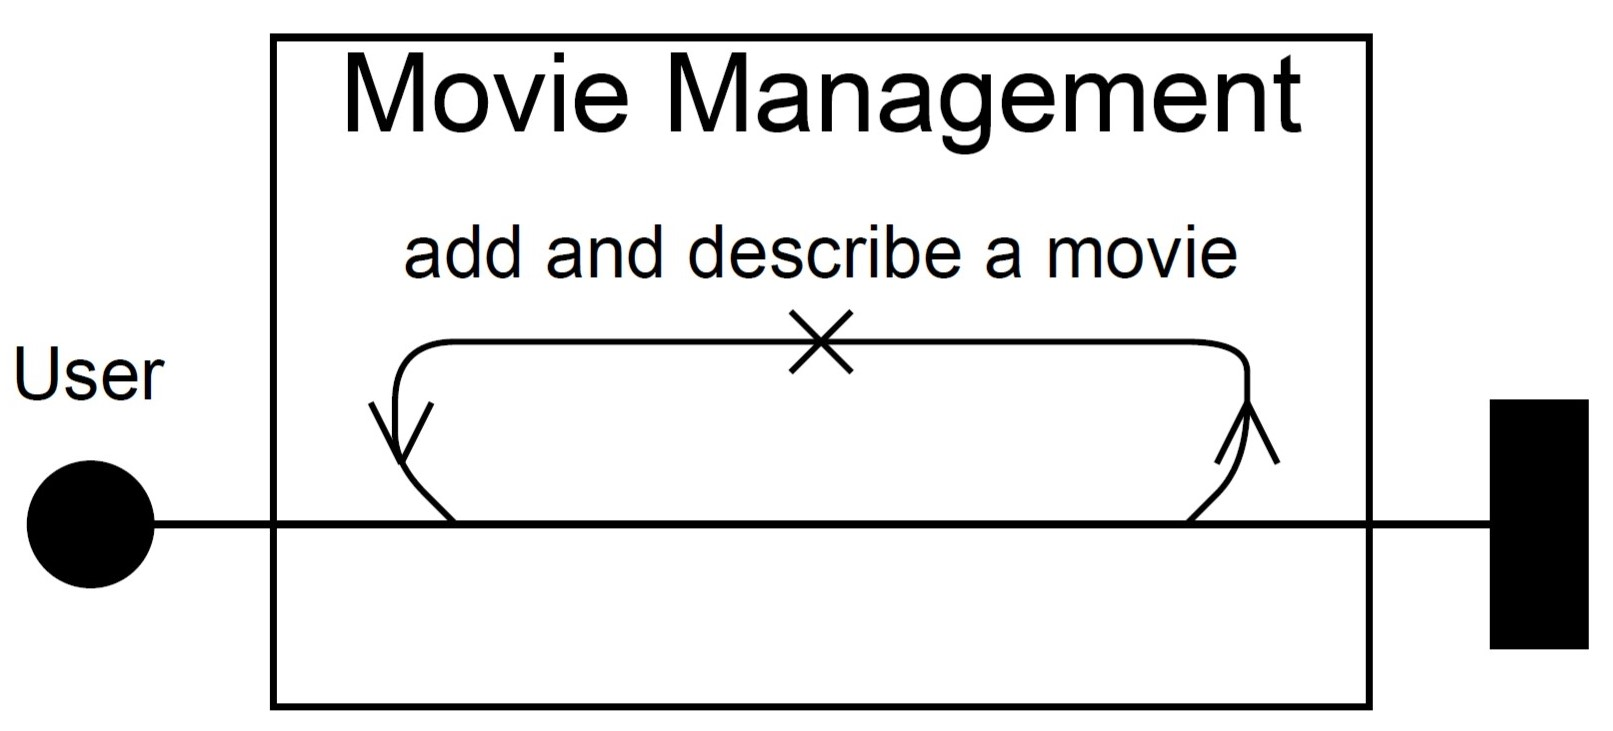
\includegraphics[scale=0.3]{../images/08/08_UCMAddAndDescribeMovie.jpg} 
	\caption{Functional Requirements in Use Case Maps Notation}
	\label{fig:08_UCMAddAndDescribeMovie}
\end{figure}
\newpage
\subsubsection{First Step: Extend the UCM}
The extended UCM is on view in \autoref{fig:08_UCMExtended}. The UCM from \autoref{fig:08_UCMAddAndDescribeMovie} is defined with information about the input
data, the expected output, a description of the behavior, and the test logic with postconditions. In this case, the function \textit{createMovie} must get as input two strings for name and country, which are not none and not empty. The generation of the input combination is described in \autoref{topic08:sectionApproach2Description}

\begin{figure}[h]
	\centering
	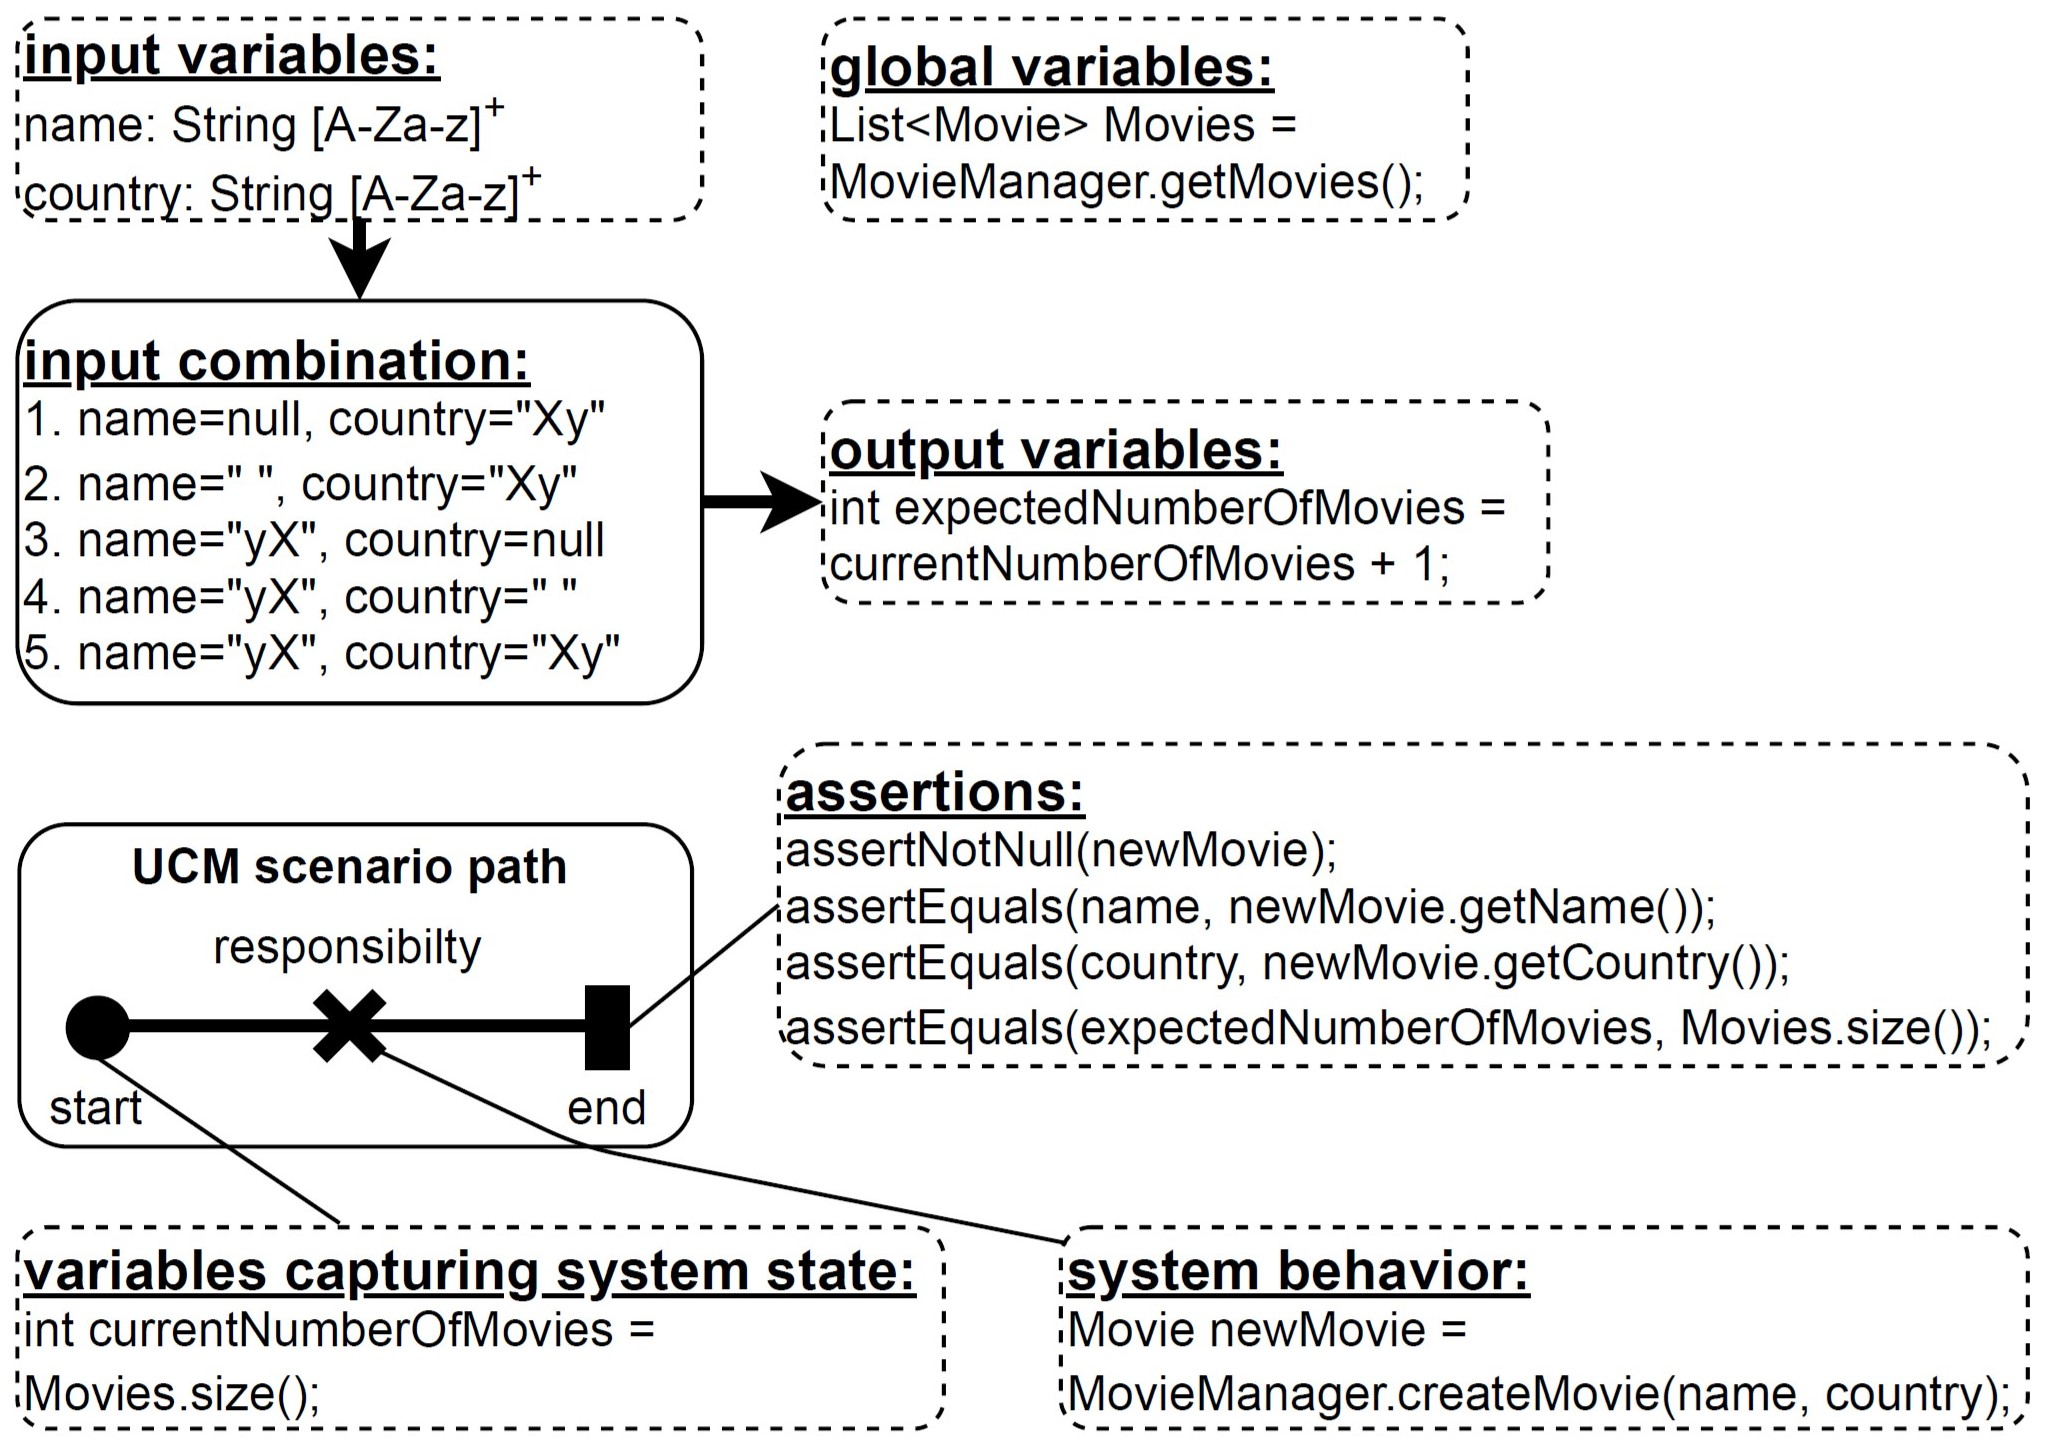
\includegraphics[scale=0.5]{../images/08/08_UCMExtended.jpg} 
	\caption{Extended Use Case Map}
	\label{fig:08_UCMExtended}
\end{figure}

\subsubsection{Second Step: Run traversal mechanism}
The acceptance test cases are now automatically generated from this extended UCM model with the traversal mechanism. Result in \autoref{lst:08_testcases}. The traversal mechanism traveling through the Use Case Map from \autoref{fig:08_UCMExtended}, from the start point to an endpoint by visiting the responsibilities and create automatically a test case skeleton which is used with the input combinations to create the specific acceptance test cases. In this case, four invalids and one valid test case.

\lstinputlisting[caption={JUnit test cases}, label={lst:08_testcases}]{../images/08/08_JUNIT.java}

\subsubsection{Third Step: Run JUnit Testing Framework}
Now, the JUnit Testing Framework can execute the acceptance tests.
%--------------------------------------------------------------------------------%
%--------------------------------------------------------------------------------%
\newpage
\section{Comparison}
\label{topic08:sectionComparison}

The approaches have been compared using a set of synthesis questions, as shown in \autoref{tab:08_syntheseMatrix1} and \autoref{tab:08_syntheseMatrix2}

Both approaches start with the User Requirements Notation. Approach one deals with the functional and non-functional requirements, whereas approach two only deals with the functional requirements. Nevertheless, in both cases, one must process the User Requirements Notation manually. In the first, the User Requirements Notation has to be transferred to the Testable Requirements Model. In the second, the Use Case Maps must be extended. In theory, the transfer to the Testable Requirements Model is more time-consuming than the extension. However, approach one has the advantage of testing the non-functional requirements as well. From this point, everything is automated. The first approach starts with the Validation Framework, which connects the Testable Requirements Model and the implementation under test, executes the test cases, collects information, and creates the Contract Evaluation Report. The second approach generates the acceptance test cases with the traversal mechanism and runs the test cases with JUnit. A significant difference is that after \textit{Arnold et al.}, the information was evaluated and written in a report, whereas after \textit{Boucher} and \textit{Mussbacher}, the result only includes which acceptance test cases are successful and which not. Therefore, the first one provides more information. Both help the stakeholder and developer in the testing process and creates a time advantage compared to the manual test creation. If one wants to test automatically functional and non-functional requirements, one has to use method one. However, both ways can be used if only the functional requirements are in question.

\newpage
\newgeometry{margin=1cm}
\begin{landscape}
	\begin{table}
		\caption{Synthesis Matrix part 1/2.}
		\begin{longtable}[h]{|p{1.3cm}|>{\raggedright}p{2.8cm}|>{}p{9.1cm}|>{}p{9.1cm}|}
			\hline
			Question 
			& Name 
			& Approach 1: \textbf{Scenario-Based Validation Beyond the User Requirements Notation} 
			& Approach 2: \textbf{Transforming Workflow Models into Automated End-to-End Acceptance Test Cases}\\ \hline
			%\hline %%%%%%%%%%%%%%%%%%%%%%%%%%%%%%%%%%%%%%%%%%%%%%%%%%%%%%%%
			\multirow{3}{*}{1 \rotatebox[origin=r]{90}{\textbf{Description}}} 
			& a) artefacts and relationship between artefacts 
			&- "Implementation under test" (IUT): Part of the software to be tested. 
			
			- "User Requirements Notation" (URN): Notation for functional requirements (FRs) and non-functional requirements (NFRs). The FRs are written in "Use Case Maps" and the NFRs in "Goal-oriented requirements Language".
			
			- "Testable Requirements Model" (TRM): Generate test cases for FRs and NFRs. Enable traceability while linking its elements to related elements of an IUT. It is written in its language "Another Contract Language". 
			
			- URN and TRM are semantically similar.
			
			- "Contract Evaluation Report" (CER): Report with all Information. The output of the VF.
			&- "Use Case Maps" (UCM): Part of the User Requirements Notation. Notation for functional requirements (FRs).
			
			- "Extended UCM": Include scenario groups, which are defined with global settings and information about setup and tear down. A scenario group consists of several scenario definitions, and every definition corresponds to a use case, which should be tested. The scenario definitions need information about the input data type, the input data, and the expected output.
			\\
			\cline{2-4}
			& b) preconditions/ input 
			&  - FRs and NFRs in URN
			
			- IUT
			& 
			- FRs in URN \\
			\cline{2-4}
			& c) steps, results, informations 
			& - The requirements must be converted manually from the URN to the TRM.
			
			- The VF must be started. VF calls the ABE for the automated binding process. VF runs the IUT, tests the behavior of the IUT with the test cases, collects and evaluates the information, and creates the CER.
			&
			- The UCM must be extended with information about scenario groups, scenario definition, start-/endpoints, and responsibility.
			
			- The UCM traversal mechanism creates the acceptance test cases by traverse the extended UCM.
			
			- "JUnit Testing Framework": Execute the acceptance tests on the software.
			\\
			\hline %%%%%%%%%%%%%%%%%%%%%%%%%%%%%%%%%%%%%%%%%%%%%%%%%%%%%%%%
			\multirow{3}{*}{2 \rotatebox[origin=r]{90}{\textbf{Benefits}}} 
			& a) supported usage scenarios 
			& - The testing process for the FRs and NFRs is automated, and there is traceability between the test cases and the IUT. 
			& - The testing process for the FRs is automated. \\ 
			\cline{2-4}
			& b) supported stakeholders 
			& - All stakeholders who are responsible for testing the software, both internal and external stakeholders.
			& - All stakeholders who are responsible for testing the software, both internal and external stakeholders.\\ 
			\cline{2-4}
			& c) corresponding SWEBOK-Knowledge Areas
			& - Software Requirements: 1.3 Functional and Nonfunctional Requirements, 6.3 Model Validation
			
			- Software Testing: 3.6 Model-Based Testing Techniques, 6.1 Testing Tool Support
			
			- Software Engineering Models and Methods: 1.4 Preconditions, Postconditions and Invariants, 2.2 Behavioral Modeling, 3.4 Traceability 
			&
			- Software Requirements: 1.3 Functional and Nonfunctional Requirements, 6.4 Acceptance Test
			
			- Software Testing: 3.6 Model-Based Testing Techniques
			
			Software Engineering Models and Methods: 1.4 Preconditions, Postconditions and Invariants\\
			\hline %%%%%%%%%%%%%%%%%%%%%%%%%%%%%%%%%%%%%%%%%%%%%%%%%%%%%%%%
		\end{longtable}
		\label{tab:08_syntheseMatrix1}
	\end{table}
\end{landscape}
\restoregeometry

\newpage
\newgeometry{margin=1cm}
\begin{landscape}
	\begin{table}
		\caption{Synthesis Matrix part 2/2.}
		\begin{longtable}[h]{|p{1.3cm}|>{\raggedright}p{2.6cm}|>{}p{9.2cm}|>{}p{9.2cm}|}
			\hline
			Question 
			& Name 
			& Approach 1: \textbf{Scenario-Based Validation Beyond the User Requirements Notation} 
			& Approach 2: \textbf{Transforming Workflow Models into Automated End-to-End Acceptance Test Cases}\\ \hline
			%\hline %%%%%%%%%%%%%%%%%%%%%%%%%%%%%%%%%%%%%%%%%%%%%%%%%%%%%%%%
			\multirow{2}{*}{3 \rotatebox[origin=r]{90}{\textbf{Tools}}} 
			& a) tool support 
			& - "Automated Binding Engine" (ABE): Automate the binding process between the elements of the TRM and the related elements of an IUT
			
			- "Validation Framework" (VF)$^*$: Get the IUT and the TRM. Call ABE to bind the elements of TRM and IUT. Run the IUT, test the behavior of the IUT with the test cases from TRM. Collect information about the input, the behavior, and the output. Evaluate the information with the metric evaluator and create the CER.
			& 		
			- "UCM traversal mechanism" from "jUCMNav tool"$^\nabla$: Traverse the extended UCM and create the acceptance test cases.
			
			- "JUnit Testing Framework": Execute the acceptance tests on the software.$^\dagger$\\ 
			\cline{2-4}
			& b) level of automation 
			& - The conversion from the URN to the TRM must be done manually without tool support. It requires a person who is familiar with a) the semantic of ACL, b) the test case generation process, and c) the binding process between IUT and TRM.  
			
			- The binding process, the execution of the IUT, the test process, and the report creation is all automated by the VF.
			& 
			- The extending of the UCM must be done manually.
			
			- The UCM traversal mechanism automates the acceptance test generation from the extended URM.
			
			- "JUnit Testing Framework" execute the acceptance tests automatically.
			\\
			\cline{2-4}
			\hline %%%%%%%%%%%%%%%%%%%%%%%%%%%%%%%%%%%%%%%%%%%%%%%%%%%%%%%%
			\multirow{2}{*}{4 \rotatebox[origin=r]{90}{\textbf{Quality}}} 
			& a) evaluation
			& - The authors did not evaluate the approach. 
			& - They have compared the lines of codes of the extending process with the lines of codes of the manually generated test cases. This was made on example software. 
			\\
			\cline{2-4}
			& b) evaluation results 
			&- The authors did not evaluate the approach. &
			- They need 60 lines of code to extend the UCM and 600 lines of code for the manual test case creation. \\
			\cline{2-4}
			\hline %%%%%%%%%%%%%%%%%%%%%%%%%%%%%%%%%%%%%%%%%%%%%%%%%%%%%%%%
		\end{longtable}
		\qquad \qquad *: The VF is developed by one of the authors, Dave Arnold, for his Ph.D. Thesis. According to the paper, the VF can be found under http://vf.davearnold.ca/.\\
		\null \qquad \qquad \quad Unfortunately, Dave Arnold's website is offline, and we didn't find a copy of the VF on the internet. Under the following link, one can see the user guide of the \\
		\null \qquad \qquad \quad VF https://www.yumpu.com/en/document/read/39418604/user-guide-validation-framework-dave-arnold \\
		\null \qquad \qquad $\nabla$: According to the paper, the "jUCMNav tool" can be found under http://jucmnav.softwareengineering.ca/jucmnav. Unfortunately, the website is unreachable, \\
		\null \qquad \qquad \quad "jUCMNav tool" can be found on https://github.com/JUCMNAV.\\
		\null \qquad \qquad $\dagger$: https://junit.org/junit5/
		\label{tab:08_syntheseMatrix2}
	\end{table}
	
\end{landscape}
\restoregeometry
%--------------------------------------------------------------------------------%
%--------------------------------------------------------------------------------%
\section{Conclusion}

This chapter acquaints two approaches to automatically generating test cases for functional and non-functional requirements from User Requirements Notation. There is a lot of potential behind this idea, but unfortunately, as one can see in the literature research, this topic has not been researched enough. Perhaps this is due to the fact that one can not directly generate the test cases automatically from the User Requirements Notation. Instead, one has to do an intermediate step and learn that this extra effort is worthwhile because the developers save time by the test case generation and improve the testing process, which results in better software quality. 

Unfortunately, the approach by \textit{Arnold et al.} is the only one that addresses functional and non-functional requirements. The problem here is that the Validation Framework can not be found on the web because the link\footnote{http://vf.davearnold.ca/} from the paper to the website is not available. However, with "Wayback Machine - Internet Archive"\footnote{http://web.archive.org/} a copy of the website\footnote{https://web.archive.org/web/20161017193123/http://vf.davearnold.ca/} is available. Additionally, under this copy, one can not download the Validation Framework, and without it, this approach does not work.  

As stated, the approach by \textit{Boucher} and \textit{Mussbacher} only generates test cases for functional requirements. The frameworks, jUCMNav\footnote{https://github.com/JUCMNAV} and JUnit\footnote{https://junit.org/junit5/}, which are needed for the approach, are available on the web. The whole process can be done quickly without problems and is recommendable.

If one wants to focus on the non-functional requirements, it can be found in the chapter \textit{"Testing non-functional requirements with risk analysis"} and \textit{"Testing non-functional requirements with aspects"}.
